\subsection*{ГЛ11 5}
Пусть изначально имеются точки $X,Z$. Проведем прямые $a_1,a_2$ так, что расстояние от каждой из них до точек $X,Z$ не больше длины линейки. Отметим $B_1$ и проведем прямые $B_1X, B_1Z$, обозначим $B_1X \cap a_2 = A_2,\ B_1Z \cap a_2 = C_2$. Отметим точку $A_1$ и проведем $A_1X, A_1C_2$, обозначим $A_1X \cap a_2 = B_2,\ B_2Z \cap a_1 = C_1,\ C_1A_2 \cap A_1C_2 = Y$. Тогда по теореме Паппа $X,Y,Z$ на одной прямой, тогда, проведя прямую $XY$ мы построим и $XZ$.\\
Если мы не можем соединить какие-то 2 точки, то повторяем данный алгоритм для них.   
\begin{figure}[h]
	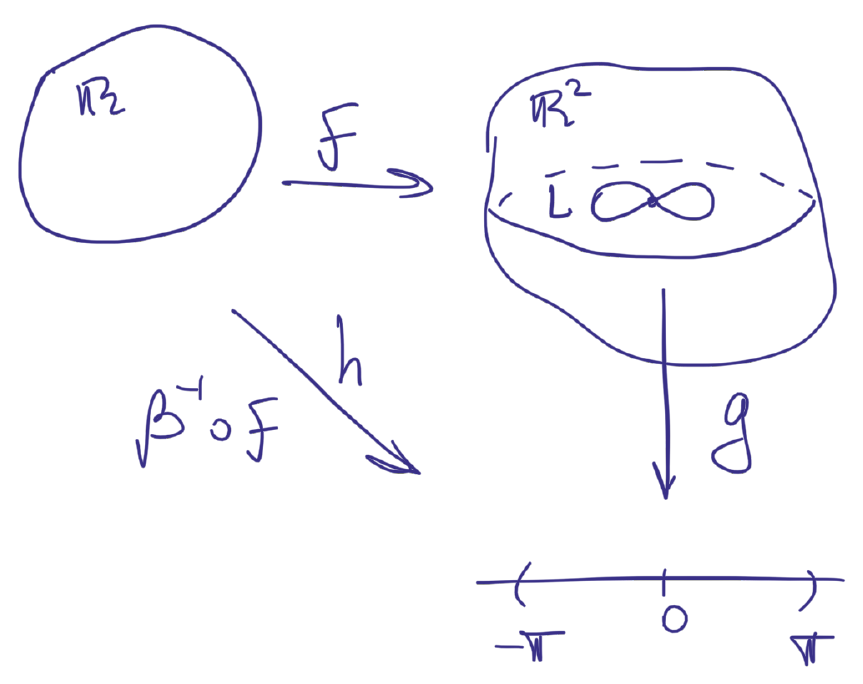
\includegraphics[width=0.5\linewidth]{pic10}
\end{figure}